\section{The leading-soft pole on the principal-series boundary}
\label{sec:boundary}
The displaced-line norm does not apply to a contour passing through a pole.
We now supply a separate statement in a specified distribution topology.
Use the Fourier convention
\[
 \mathcal F_+h(\nu)=\int_{\mathbb R}e^{i\nu t}h(t)\,dt.
\]
For a distribution $T$ in the variable $\nu$, define the standard inhomogeneous
negative Sobolev norm by
\[
 \|T\|_{H^{-q}}^2=\frac1{2\pi}\int_{\mathbb R}
 (1+t^2)^{-q}|\mathcal F_-T(t)|^2\,dt,
\]
when its Fourier transform is a function and the integral is finite.

\begin{theorem}[Boundary instability with an exact norm]\label{thm:boundary}
For the family of Theorem~\ref{thm:instability}, set
\[
 h_N(t)=c(1+e^t/R)^{-N},\qquad T_N=\mathcal F_+h_N.
\]
For each fixed $N$, the boundary limit
$F_N(p+\varepsilon+i\nu)\to T_N$ exists in the tempered distributions
as $\varepsilon\downarrow0$. For every $q>1/2$,
\begin{align}
 \|T_N\|_{H^{-q}}^2
 &=2\pi c^2\int_{\mathbb R}(1+t^2)^{-q}(1+e^t/R)^{-2N}\,dt
 \longrightarrow0,\label{eq:boundarynorm}\\
 \|T_N\|_{H^{-q}}^2
 &\sim \frac{2\pi c^2}{2q-1}(\log N)^{1-2q}.
 \label{eq:boundaryrate}
\end{align}
The residue at $p$ remains $c$. For $q\le1/2$, $T_N$ has infinite
$H^{-q}$ norm for every $N$. In particular, $p=1$ gives instability
on the four-dimensional leading-soft principal-series contour in each
of the stated $H^{-q}$ topologies.
\end{theorem}
\begin{proof}
The change of variables $\omega=e^t$ gives
$F_N(p+\varepsilon+i\nu)=\mathcal F_+(e^{\varepsilon t}h_N)$.
For $t\le0$ and $0<\varepsilon\le N/2$, the absolute value is at most $c$.
For $t\ge0$ it is at most $cR^Ne^{-Nt/2}$.
Pairing with any Schwartz test function and dominated convergence therefore
prove the Abel boundary limit. Since $\mathcal F_-\mathcal F_+h_N=2\pi h_N$,
the norm identity follows. Its integrand tends pointwise to zero and is
bounded by the integrable function $(1+t^2)^{-q}$ if $q>1/2$.
If $q\le1/2$, $h_N(t)\to c$ as $t\to-\infty$ forces divergence.

For the asymptotic, put $\ell=\log N$ and fix $0<\epsilon<1$.
On $t\le-(1+\epsilon)\ell$ the profile factor tends uniformly to one.
On $t\ge-(1-\epsilon)\ell$ it is at most
$(1+N^{-1+\epsilon}/R)^{-2N}$, which is exponentially small in $N^\epsilon$.
Split the integral at these two locations and use
\[
 \int_{-\infty}^{-b\ell}(1+t^2)^{-q}\,dt
 \sim \frac{(b\ell)^{1-2q}}{2q-1},\qquad b>0.
\]
The lower and upper asymptotic constants are squeezed between
$(1+\epsilon)^{1-2q}/(2q-1)$ and
$(1-\epsilon)^{1-2q}/(2q-1)$. Let $\epsilon\downarrow0$.
\end{proof}

The midpoint argument of Corollary~\ref{cor:discontinuous} now applies
with $H^{-q}$ error balls and again gives residue error at least $c/2$.
The result also holds for pairs $T_{N_0}+T_N$ and $T_{N_0}$, so it does
not require a zero profile. This is a topology-dependent instability of
extraction; it does not contradict completeness of the principal-series
basis or exact contour representations of soft modes
\cite{basis,asymptotic}. The use of distributions in celestial amplitudes
has an established mathematical treatment \cite{distributional}.

\section{Direct Mellin-data recovery and an optimal error exponent}
\label{sec:direct}
The energy-window theorem below assumes stronger observations than
Mellin-line data. Here we instead construct an estimator directly from
the latter. A uniform infrared modulus is the additional prior.
Work in a fixed numerical energy convention and strip a known power:
$A(x)=x^{-p}f(x)$, so $G(z)=\Mell A(p+z)$.
For $a,\alpha,M>0$, let $\mathcal C_{a,\alpha,M}$ consist of continuous
complex functions on $[0,\infty)$ satisfying
\begin{equation}\label{eq:holderclass}
 |f(x)-f(0)|\le Mx^\alpha\quad(x>0),\qquad
 Q_a(f):=\int_0^\infty x^{a-1}|f(x)|\,dx<\infty.
\end{equation}
The modulus is global as written. A bound restricted to an infrared
interval would require an additional ultraviolet-tail term for the
Gaussian estimator. The infrared expansion and the ultraviolet
integrability in \eqref{eq:holderclass} give a meromorphic continuation
near $z=0$, with residue $r=f(0)$: split the integral at one, subtract
$r$ in the infrared, and continue that remainder to $\Re z>-\alpha$.
The ultraviolet integral is holomorphic in $\Re z<a$.

\begin{theorem}[Direct recovery; matching minimax exponent]\label{thm:direct}
Observe the complete line $Y(\nu)=G(a+i\nu)+e(\nu)$, with measurable
$\|e\|_\infty\le\eta$. For $h>0$, define
\begin{equation}\label{eq:estimator}
 \widehat r_h(Y)=\frac1{2\pi}\int_{\mathbb R}
 Y(\nu)h^{-a-i\nu}\exp\big((a+i\nu)^2/2\big)\,d\nu.
\end{equation}
Put $A_\alpha=e^{\alpha^2/2}$ and $B_a=e^{a^2/2}/\sqrt{2\pi}$.
For every $f\in\mathcal C_{a,\alpha,M}$,
\begin{equation}\label{eq:directbound}
 |\widehat r_h-r|\le A_\alpha Mh^\alpha+B_a\eta h^{-a}.
\end{equation}
Let $\mathcal R(\eta)$ be the minimax worst-case absolute error over
this class and these noise balls. With
$\theta=\alpha/(a+\alpha)$, there are explicit constants depending
only on $a,\alpha$ such that
\begin{equation}\label{eq:minimaxrate}
 c_{a,\alpha}M^{a/(a+\alpha)}\eta^\theta
 \le\mathcal R(\eta)\le
 C_{a,\alpha}M^{a/(a+\alpha)}\eta^\theta,
\end{equation}
where
\begin{align*}
 c_{a,\alpha}&=\tfrac12
 \left(\frac{2\alpha}{\Gamma(a/\alpha)}\right)^\theta,\\
 C_{a,\alpha}&=A_\alpha^{a/(a+\alpha)}B_a^\theta
 \left[(a/\alpha)^\theta+(\alpha/a)^{a/(a+\alpha)}\right].
\end{align*}
Thus the exponent is optimal; equality of the two constants is not asserted.
\end{theorem}
\begin{proof}
Absolute convergence follows from $|G(a+i\nu)|\le Q_a(f)$ and the
Gaussian factor. Fubini is justified by the same bound. The elementary
Gaussian Fourier integral gives the identity
\begin{equation}\label{eq:gaussianidentity}
 \widehat r_h(G)=\frac1{\sqrt{2\pi}}\int_{\mathbb R}
 e^{-t^2/2}f(he^t)\,dt.
\end{equation}
For example, the inner frequency integral after interchanging the
energy and frequency integrals equals
$h^{-a}e^{a^2/2}\exp[-(\log(x/h)+a)^2/2]/\sqrt{2\pi}$;
the change $x=he^t$ yields \eqref{eq:gaussianidentity}.
The modulus in \eqref{eq:holderclass} bounds its bias by
$Mh^\alpha\mathbb E e^{\alpha Z}=A_\alpha Mh^\alpha$ for standard
normal $Z$. The $L^1$ norm of the frequency kernel in
\eqref{eq:estimator} is exactly $B_ah^{-a}$, giving the noise term.
For $M,\eta>0$, choose
\[
 h_* = \left(\frac{aB_a\eta}{\alpha A_\alpha M}\right)^{1/(a+\alpha)}.
\]
Substitution proves the upper constant. If $\eta=0$, take $h\downarrow0$.

For the lower bound, compare zero to the nonnegative profile
\[
 f_c(x)=c\exp[-(M/c)x^\alpha],\qquad c>0.
\]
Since $1-e^{-u}\le u$ for $u\ge0$, this profile belongs to the class.
Its transform is
\[
 G_c(z)=\frac{c}{\alpha}(c/M)^{z/\alpha}\Gamma(z/\alpha),
 \quad
 \|G_c\|_{a,\infty}=\frac{\Gamma(a/\alpha)}{\alpha}
 c^{1+a/\alpha}M^{-a/\alpha}.
\]
The norm equality follows directly from positivity and equality at
$\nu=0$. Choose
$c=[2\alpha\eta M^{a/\alpha}/\Gamma(a/\alpha)]^\theta$.
The common observation $G_c/2$ is then within $\eta$ of both transforms.
Their residues differ by $c$, so every estimator has error at least $c/2$.
\end{proof}

For $\alpha=1$ the lower-bound profiles are completely monotone.
The optimal square-root rate at $a=\alpha=1$ is especially explicit:
\begin{equation}\label{eq:sqrtrate}
 \frac1{\sqrt2}\sqrt{M\eta}\le\mathcal R(\eta)
 \le \frac{2\sqrt e}{(2\pi)^{1/4}}\sqrt{M\eta}.
\end{equation}
The regularity assumption constrains the shrinking transition scale
that was unrestricted in Theorem~\ref{thm:instability}.
These elementary Gaussian regularization and two-point minimax
arguments should not be construed as a new general inverse-problem
principle. Extrapolation with complete monotonicity has close prior work
\cite{brown}; the observation operator and norms there differ from ours.

\begin{corollary}[A finite frequency band]\label{cor:band}
If observations are restricted to $|\nu|\le\Omega$ and the prior also
supplies $Q_a(f)\le Q$, truncate \eqref{eq:estimator} to this band.
Then
\[
 |\widehat r_{h,\Omega}-r|\le A_\alpha Mh^\alpha+
 B_ah^{-a}\left[\eta+Q\operatorname{erfc}(\Omega/\sqrt2)\right].
\]
Here the noise is bounded on a continuum band. Discrete sampling and
numerical quadrature introduce additional errors not bounded by this statement.
\end{corollary}
\begin{proof}
The omitted exact-data contribution is at most
$Q B_ah^{-a}\operatorname{erfc}(\Omega/\sqrt2)$ by the Gaussian tail
integral. The in-band noise contributes at most $B_a\eta h^{-a}$.
Add the bias bound from Theorem~\ref{thm:direct}.
\end{proof}

Theorems~\ref{thm:boundary} and \ref{thm:direct} use different data
models: a distribution on the boundary line in the first, and bounded
noise on a displaced, absolutely convergent line in the second.
Neither theorem transfers an error bound between those models.
Together they specify an obstruction and a conditional recovery result,
while leaving the physical scattering subclass and broader celestial
holography questions open.

\begin{figure}[ht]
\centering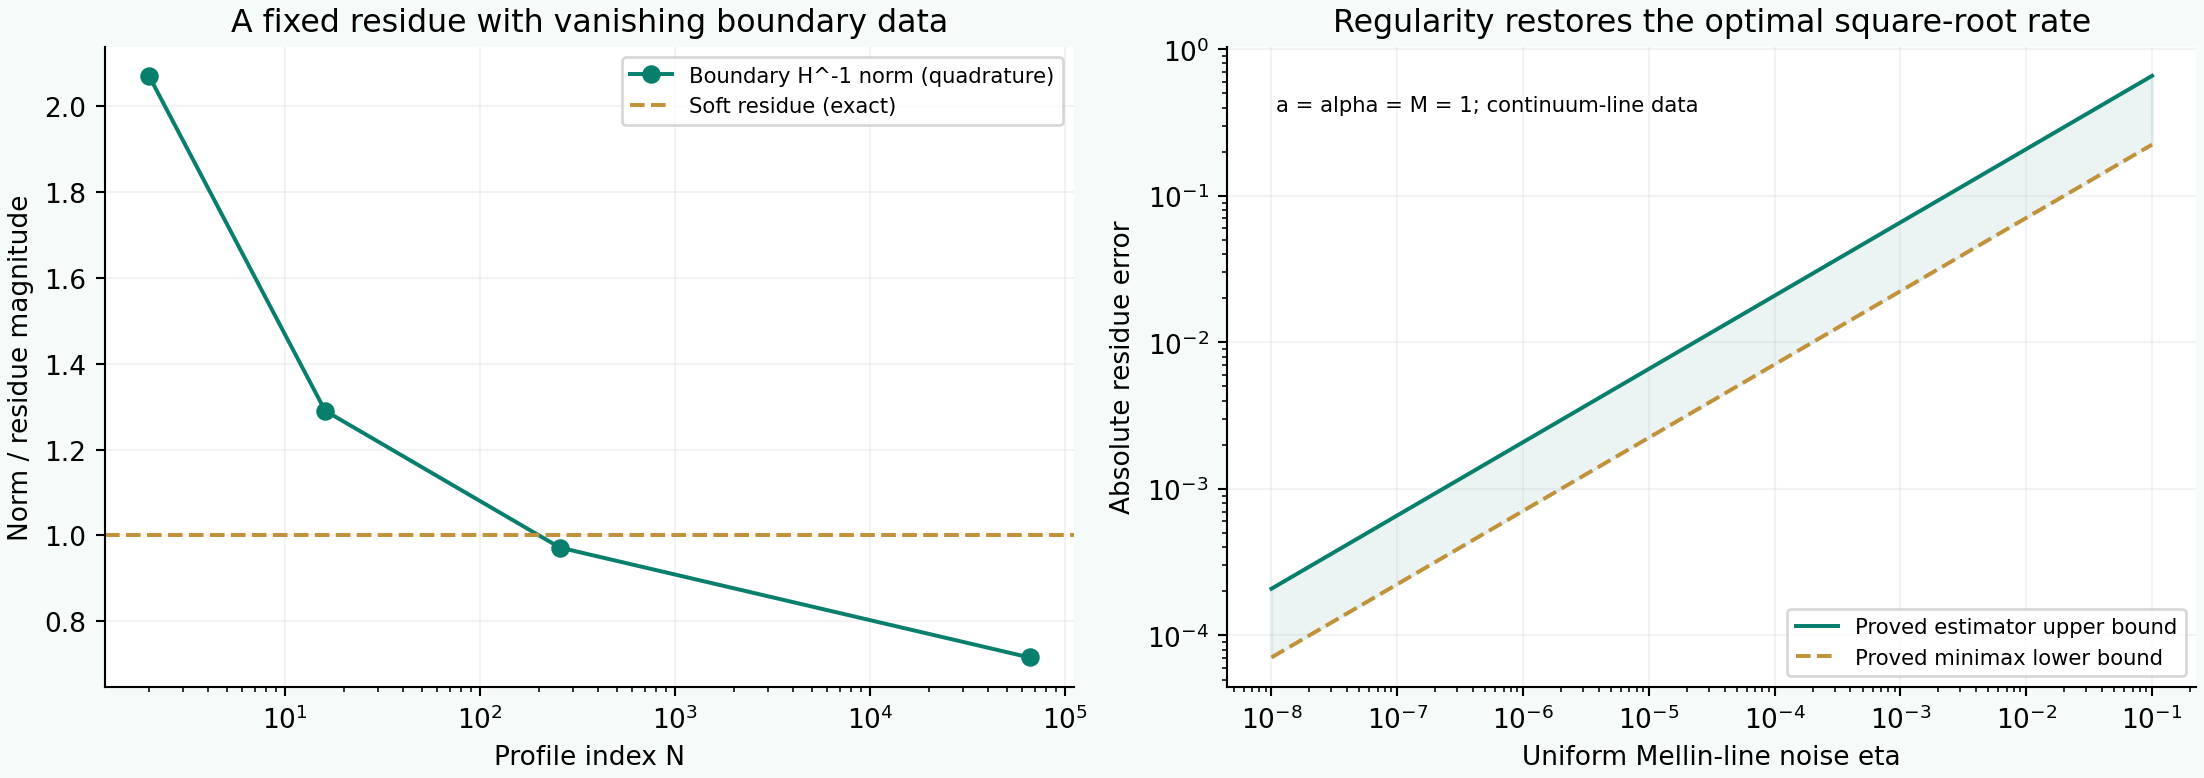
\includegraphics[width=\linewidth]{assets/stability-tradeoff.png}
\caption{Left: numerical evaluations of the exact boundary norm for
$q=c=R=1$, with the exact fixed residue shown separately.
Right: proved upper and lower direct-data recovery bounds at
$a=\alpha=M=1$. The matching exponent does not assert equal constants.
The panels concern different data norms.}
\end{figure}
